\subsection{Introduction}
\label{subsec:introduction}
Deep neural networks are usually composed of sequential interconnected layers.
This structure allows for extreme parallelism as computations are broken into smaller chunks, albeit still dependent on its previous layers.
Each layer in a neural network takes in an activation tensor as well as a weight tensor.
An activation tensor represents the output of a single node in the layer, while a weight tensor represents the learning parameters in the network.
The computation between the two tensors involves a mathematical expression similar to matrix multiplications, outputting an activation tensor fed on to the next layer.

\subsection{SM Core}
\label{subsec:sm-core}
The structure of the A100's SM core works via a 5-step process.
The A100's memory hierarchy starts with the off-chip DRAM\@.
The DRAM provides global access to resources for the SMs.
Data is first loaded from the DRAM into the on-chip L2 cache, acting as a large pool of shared memory accessible by all SMs.
An asynchronous instruction will then be used to partition the data resource for SMEM usage individually and concurrently without blocking the main execution pipeline.
Think of the instruction as an asynchronous implicit duplicate instruction that allows data to be loaded directly from the main memory into a shared memory.
The SMEM connects to the tensor cores via a register file, which acts as a high-speed buffer location, allowing tensor cores to efficiently read and write data to and from the SMEM\@.

\begin{figure}[htbp!]
    \centerline{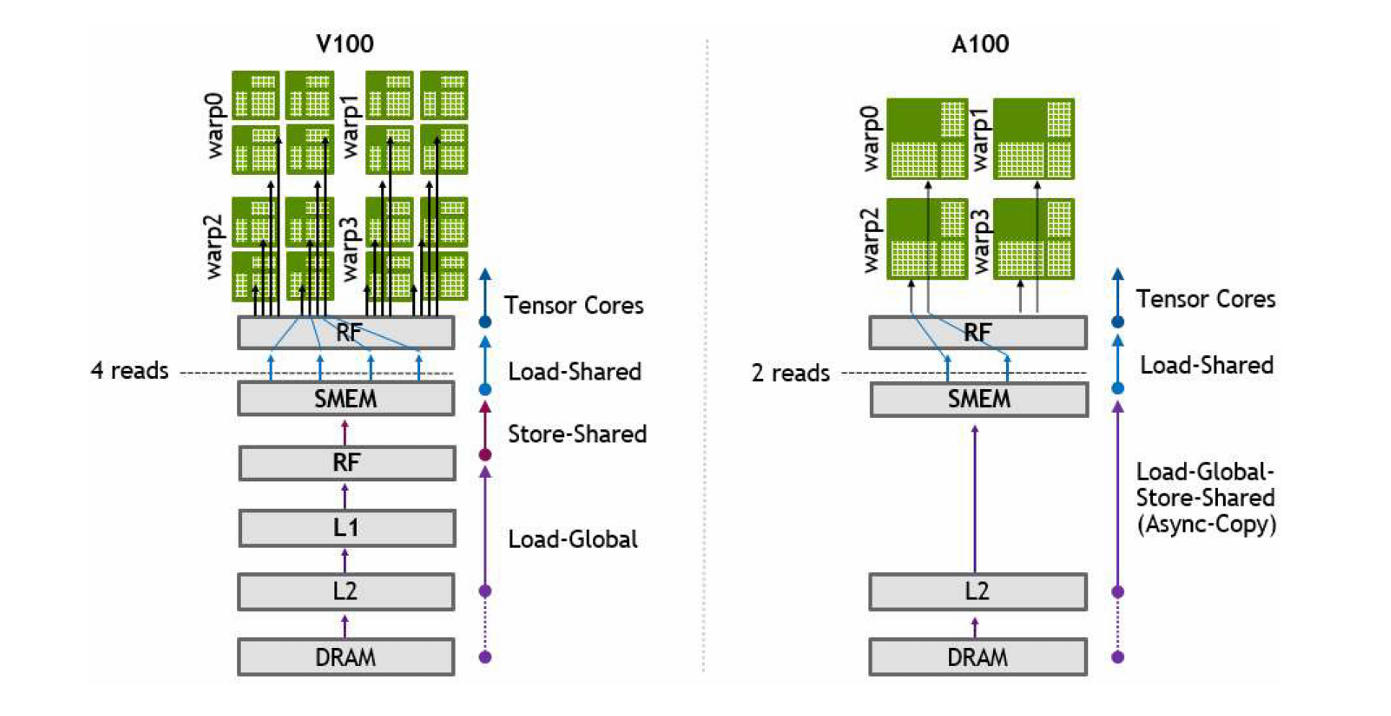
\includegraphics[width=0.5\textwidth]{images/gpu_structure}}
    \caption{V100 vs. A100 structure.}
    \label{fig:v100a100struct}
\end{figure}

To provide context for the specific design of the A100, its predecessor, the V100 can be examined.
The V100 works with a 7-step process.
In the same fashion, data is loaded into an L2 cache from the DRAM, but instead of a direct connection to the SMEM, the V100 requires an additional layer of caching.
By having a dedicated L1 cache per SM, the V100 can make better use of the available memory bandwidth.
Each SM can access its own L1 cache independently, reducing contention and improving overall throughput.
The V100 lacks the asynchronous ``load and store'' instruction in its instruction set; thus it requires an explicit ``write'' instruction to the SMEM to transfer data.

\begin{figure}[htbp!]
    \centerline{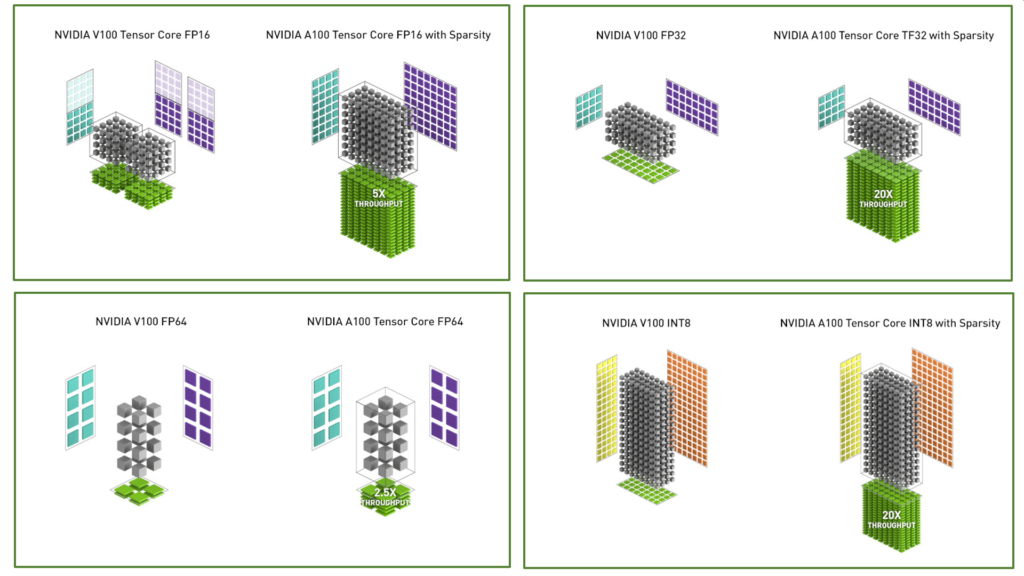
\includegraphics[width=0.5\textwidth]{images/gpu_sparsity}}
    \caption{V100 vs. A100 sparsity.}
    \label{fig:v100a100spars}
\end{figure}

The simplification of the V100 design into the A100 is actually caused by the massive throughput of the tensor core itself.
In both the V100 and A100 designs, the neural network workloads break down each tile into four smaller workable tiles that can be processed in parallel.
A 32-thread warp will then process each of those tiles.
The V100 tensor cores were designed to work with 8-thread granularity, meaning each tensor core operation would process eight threads simultaneously, while the A100 works with 32-thread granularity.
``Fig. \ref{fig:v100a100struct}'' shows the structure of the V100 and A100, while ``Fig. \ref{fig:v100a100spars}'' shows the sparsity of the V100 and A100, comparing the V100’s and A100’s standard operation with multiple data types.
The data types given such as TF32 and TF16 are much more efficient in using tensor-accelerated math than its floating point counterparts, having the same exponent range, albeit less precision.

The 8-thread granularity of the V100's individual network tiles forces it to have a proportionally higher number of load from memory and lower bandwidth in the SMEM, since the 8-thread granularity combined with the fact that data has to move from the L2 cache, to the L1 cache and then to the SMEM, results in higher number of memory access operations per tile.
Reorganizing the A100 to use 32-thread granularity allows it to process a full warp of 32 threads all at once, coupled with improvements in memory access, changed the memory access count from 1 L1 read, 1 SMEM write and 4 SMEM reads into just two SMEM reads per tile.
This reduction in memory access simplifies the data path by relying more on the higher bandwidth SMEM connecting directly without intermediary storage.

\subsection{L2 Cache}
\label{subsec:l2-cache}
An L2 cache in the A100 is a globally shared resource for the SMs.
The A100 divides its L2 cache partitions into two distinct partitions: high-bandwidth access and low latency memory access.
The cache allows for a significant increase in machine learning workloads, with larger datasets and models now being able to be cached and repeatedly hit, contrasting to the V100 requiring slower reading and writing, from and to the HBM2 memory.
The prime enabler of the partition is the L2 Cache Residency Control.
The residency control basically enables a partition of the cache to be used for persistent data access.The A100 employs two key mechanisms to manage persistent accesses to the L2 cache:

\subsubsection{Address-based Persistent Window} Specified address range or “window” will be cached instead of caching a single address and designated to be resident.
Read and write access would be a guaranteed hit in the window.
This method benefits from array-like or consecutive structures such as neural network parameters.

\subsubsection{Per-Memory-Operation Persistent Control} The residency control exposes control over Individual memory accesses to be tagged as persistent by the user, otherwise individual access will not be tagged.
These two persistent access mechanisms work together to optimize the utilization of the L2 cache.
Cache Residency only allows cache tagging when there is ``group access'' to a particular address at a close time, while individual memory access will bypass cache, or can be controlled directly by user to persist.

\subsection{DRAM}
\label{subsec:dram}
The A100 DRAM uses HBM2 memory technology.
The DRAM consists of five of these HBM2 memory stacks, laid vertically and connected to the GPU die via high-speed interconnects.
The tight integration reduces memory latency, power consumption, and its compact stack design aids in the memory having a smaller physical footprint compared to traditional GDDR memory.

\subsection{Closing}
\label{subsec:closing}
The NVIDIA A100 GPU marks a significant advancement in GPU architecture, leveraging innovative hardware designs.
From streamlining its preceding 7-step process of the SM core to a 5-step process, to including compression and residency algorithms to the cache, and introducing asynchronous partitioning instruction to enable direct data transfer to high-bandwidth SMEM\@.